\loai{Loại 1: Thế năng phân tử}
\begin{ex}
	Các phân tử cấu tạo nên vật có thế năng tương tác là do
	\choice
	{các phân tử chuyển động hỗn loạn không ngừng}
	{các phân tử chịu tác dụng của lực từ của Trái Đất}
	{các phân tử chịu tác dụng của lực hấp dẫn của Trái Đất}
	{\True giữa các phân tử có lực tương tác}
	\loigiai{
		Các phân tử cấu tạo nên vật có thế năng tương tác là do giữa các phân tử có lực tương tác. Lực tương tác này bao gồm lực hút và lực đẩy, phụ thuộc vào khoảng cách giữa các phân tử. Khi ở khoảng cách rất gần, lực đẩy trở nên mạnh mẽ, ngăn không cho các phân tử tiến lại quá gần nhau. Khi khoảng cách tăng lên chút ít, lực hút lại chiếm ưu thế, giữ các phân tử lại với nhau. Chính những lực tương tác này xác định thế năng của các phân tử.
	}
	\haidong{2}\end{ex}
\loai{Loại 2: Động năng phân tử}
\begin{ex}
	Khi nhiệt độ của vật tăng lên thì
	\choice
	{\True động năng của các phân tử cấu tạo nên vật tăng}
	{động năng của các phân tử cấu tạo nên vật giảm}
	{nội năng của vật giảm}
	{thế năng của các phân tử cấu tạo nên vật tăng}
	\loigiai{
		Khi nhiệt độ của vật tăng lên, năng lượng nhiệt của vật cũng tăng, điều này đồng nghĩa với việc động năng của các phân tử cấu tạo nên vật tăng lên do các phân tử chuyển động nhanh hơn. Nội năng của vật tăng bởi vì nó bao gồm cả động năng và thế năng của các phân tử.
	}
	\haidong{2}\end{ex}
\loai{Loại 4: Khái niệm nội năng}
\begin{ex}
	Nội năng của một vật là
	\choice
	{tổng động năng và thế năng của các vật}
	{\True tổng động năng và thế năng của các phân tử cấu tạo nên vật}
	{tổng nhiệt năng và cơ năng mà vật nhận được trong quá trình truyền nhiệt và thực hiện công}
	{nhiệt lượng vật nhận được trong quá trình truyền nhiệt}
	\loigiai{
		Nội năng của một vật là tổng động năng và thế năng của các phân tử cấu tạo nên vật. Động năng là do chuyển động nhiệt của các phân tử, trong khi thế năng là do tương tác giữa các phân tử.
	}
	\haidong{2}\end{ex}

\begin{ex}
	Nội năng của một vật
	\choice
	{chỉ phụ thuộc vào nhiệt độ của vật}
	{chỉ phụ thuộc vào thể tích của vật}
	{\True phụ thuộc vào thể tích và nhiệt độ của vật}
	{không phụ thuộc vào thể tích và nhiệt độ của vật}
	\loigiai{
		Nội năng của một vật phụ thuộc vào nhiệt độ và thể tích của nó. Nhiệt độ liên quan đến động năng của các phân tử, còn thể tích liên quan đến thế năng do tương tác giữa các phân tử.
	}
	\haidong{2}\end{ex}
\begin{ex} \nguon{1}
	Đơn vị của nội năng là
	\choice
	{W (oát)}
	{\True J (jun)}
	{A (ampe)}
	{V (vôn)}
	\loigiai{
		Đơn vị của nội năng là J (jun), vì nội năng là một dạng năng lượng, và jun là đơn vị đo năng lượng trong hệ SI.
	}
\end{ex}
\loai{Loại 5: Khái niệm nội năng. Phát biểu đúng}
\begin{ex} \nguon{3}
	Phát biểu nào sau đây nói về nội năng là đúng?
	\choice
	{Nội năng là nhiệt lượng}
	{Nội năng của vật $A$ lớn hơn nội năng của vật $B$ thì nhiệt độ của vật $A$ cũng lớn hơn nhiệt độ của vật $B$}
	{Nội năng của vật thay đổi trong quá trình truyền nhiệt, không thay đổi trong quá trình thực hiện công}
	{\True Nội năng là một dạng năng lượng}
	\loigiai{
		\begin{itemize}
			\item Nội năng là tổng động năng và thế năng của các phân tử cấu tạo nên vật.
			\item Nội năng là một dạng năng lượng nội tại của vật, không phải là nhiệt lượng.
			\item Nội năng của một vật không chỉ phụ thuộc vào nhiệt độ mà còn phụ thuộc vào trạng thái tổ chức và các thông số khác của vật.
			\item Nội năng có thể thay đổi trong quá trình truyền nhiệt và cũng có thể thay đổi trong quá trình thực hiện công.
		\end{itemize}
	}
\end{ex}
\loai{Loại 6: Khái niệm nội năng. Phát biểu sai}
\begin{ex}
	Phát biểu nào sau đây là \textbf{sai} khi nói về các cách làm thay đổi nội năng của một vật?
	\choice
	{Nội năng của vật có thể biến đổi bằng hai cách là thực hiện công và truyền nhiệt}
	{Nội năng của vật thay đổi do vật khác tác dụng lực lên vật đang xét gọi là thực hiện công}
	{Nội năng của vật thay đổi không bằng cách thực hiện công gọi là sự truyền nhiệt}
	{\True Nội năng của vật thay đổi bằng cách thực hiện công gọi là sự truyền nhiệt}
	\loigiai{
		Quá trình truyền nhiệt là quá trình làm thay đổi nội năng của một vật thông qua sự trao đổi nhiệt lượng mà không cần thực hiện công. Việc thực hiện công là quá trình thay đổi nội năng liên quan đến sự tương tác cơ học, do đó, quá trình này không phải là quá trình truyền nhiệt.
	}
	\haidong{2}\end{ex}
\loai{Loại 7: Nhiệt năng và nội năng}
\begin{ex}
	Phát biểu nào sau đây là \textbf{sai} khi nói về nhiệt lượng?
	\choice
	{\True Một vật lúc nào cũng có nội năng do nó lúc nào cũng có nhiệt lượng}
	{Đơn vị của nhiệt lượng cũng là đơn vị của công}
	{Nhiệt lượng không phải là nội năng}
	{Nhiệt lượng là phần nội năng vật tăng thêm khi nhận được nội năng từ vật khác}
	\loigiai{
		Phát biểu "Một vật lúc nào cũng có nội năng do nó lúc nào cũng có nhiệt lượng" là sai. Nội năng là tổng năng lượng bên trong của vật, luôn tồn tại. Nhiệt lượng là phần năng lượng nhiệt mà vật trao đổi với các vật khác.
	}
	\haidong{2}\end{ex}
\loai{Loại 8: Thay đổi nội năng bằng cách thực hiện công}
\begin{ex}
	Nội năng của vật bị biến đổi \textbf{không} phải do truyền nhiệt là trường hợp nào sau đây?
	\choice
	{Chậu nước để ngoài nắng một lúc thì nóng lên}
	{Gió mùa đông bắc tràn về làm cho không khí lạnh đi}
	{\True Khi trời lạnh, ta xoa hai bàn tay vào nhau cho ấm lên}
	{Cho cơm nóng vào bát thì bưng bát cũng thấy nóng}
	\loigiai{
		Khi trời lạnh và ta xoa hai bàn tay vào nhau cho ấm lên, nội năng của bàn tay tăng lên vì công cơ học đã được chuyển hóa thành nhiệt năng chứ không phải do quá trình truyền nhiệt từ môi trường bên ngoài. Các ví dụ khác đều liên quan đến sự truyền nhiệt làm thay đổi nội năng.
	}
	\haidong{3}\end{ex}
\begin{ex}
	Trường hợp nào dưới đây làm biến đổi nội năng \textbf{không} do thực hiện công?
	\choice
	{\True Đun nước}
	{Một viên bi bằng thép rơi xuống đất mềm}
	{Cọ xát hai vật vào nhau}
	{Nén khí trong xi lanh}
	\loigiai{
		Đun nước làm tăng nội năng của nước thông qua quá trình truyền nhiệt mà không cần thực hiện công cơ học nào. Trong khi đó, các quá trình còn lại (rơi xuống đất mềm, cọ xát, và nén khí) đều liên quan đến việc thực hiện công để biến đổi nội năng.
	}
	\haidong{4}\end{ex}
\loai{Loại 9: Thay đổi nội năng bằng cách truyền nhiệt}
\begin{ex}
	Khi thả một thỏi kim loại đã được nung nóng vào một chậu nước lạnh thì nội năng của thỏi kim loại và của nước thay đổi như thế nào?
	\choice
	{Nội năng của thỏi kim loại và của nước đều tăng}
	{Nội năng của thỏi kim loại và của nước đều giảm}
	{\True Nội năng của thỏi kim loại giảm, nội năng của nước tăng}
	{Nội năng của thỏi kim loại tăng, nội năng của nước giảm}
	\loigiai{
		Khi thả thỏi kim loại nóng vào nước lạnh, nội năng của thỏi kim loại sẽ truyền sang nước vì nhiệt độ thỏi kim loại cao hơn nhiệt độ của nước. Do đó, nội năng của thỏi kim loại sẽ giảm, còn nội năng của nước sẽ tăng lên, dẫn đến sự thay đổi nhiệt độ của cả hai vật.
	}
	\haidong{3}\end{ex}
\loai{Loại 10: Thay đổi nội năng bằng cách truyền nhiệt và thực hiện công}
\loai{Loại 12: Biểu thức định luật I}
\begin{ex}
	Công thức nào sau đây mô tả đúng định luật I  nhiệt động lực học?
	\choice
	{$\Delta U = A - Q$}
	{$\Delta U = Q - A$}
	{$A = \Delta U - Q$}
	{\True $\Delta U = A + Q$}
	\loigiai{
		Theo định luật I của Nhiệt động lực học, độ biến thiên nội năng ($\Delta U$) của một hệ bằng tổng cộng ($A$) mà hệ nhận được và nhiệt lượng ($Q$) mà hệ nhận được: $\Delta U = A + Q$. Trong đó:
		\begin{itemize}
			\item $\Delta U$ là độ biến thiên nội năng.
			\item $A$ là công mà hệ nhận được.
			\item $Q$ là nhiệt lượng mà hệ nhận được.
		\end{itemize}
	}
	\haidong{2}
\end{ex}
\begin{ex} \nguon{1}
	Định luật I của nhiệt động lực học là sự vận dụng của định luật bảo toàn nào sau đây?
	\choice
	{Định luật bảo toàn cơ năng}
	{Định luật bảo toàn động lượng}
	{\True Định luật bảo toàn và chuyển hóa năng lượng}
	{Định luật II Newton}
	\loigiai{
		\begin{itemize}
			\item Định luật I của nhiệt động lực học, phát biểu rằng độ biến thiên nội năng của một hệ bằng tổng của nhiệt lượng mà hệ nhận được và công mà hệ nhận được, là một sự vận dụng của định luật bảo toàn và chuyển hóa năng lượng. 
			
			\item Theo quy tắc này, năng lượng không tự sinh ra hoặc mất đi mà chỉ chuyển từ dạng này sang dạng khác và từ hệ này sang hệ khác. Định luật I của nhiệt động lực học là cụ thể hóa nguyên lí này cho các quá trình nhiệt động lực học, đảm bảo rằng tổng năng lượng (bao gồm cả nội năng, nhiệt lượng, và công) của một hệ và môi trường xung quanh là không đổi.\end{itemize}
	}
\end{ex}

\loai{Loại 13: Dấu của A, Q và Delta U}
\begin{ex}
	Theo định luật I của nhiệt động lực học có công thức $\Delta U = Q + A$. Quá trình nào sau đây diễn tả quá trình biến thiên nội năng khi hệ nhận công và truyền nhiệt lượng?
	\choice
	{$\Delta U = Q + A$ khi $Q > 0$ và $A > 0$}
	{$\Delta U = Q + A$ khi $Q > 0$ và $A < 0$}
	{\True $\Delta U = Q + A$ khi $Q < 0$ và $A > 0$}
	{$\Delta U = Q + A$ khi $Q < 0$ và $A < 0$}
	\loigiai{
		Khi hệ truyền nhiệt lượng ra ngoài, nhiệt lượng $Q$ mất đi nên $Q < 0$. Khi hệ nhận công từ môi trường, công $A$ được thêm vào hệ nên $A > 0$. Vì vậy, quá trình diễn tả biến thiên nội năng khi hệ nhận công và truyền nhiệt lượng là khi $Q < 0$ và $A > 0$.
	}
	\haidong{1}
\end{ex}
\begin{ex}%[1P6B3-1][Loai2]
	Trong quá trình chất khí tỏa nhiệt và nhận công thì dấu của A và Q trong biểu thức $\Delta U = A+Q$ là
	\choice
	{$Q > 0,\ A < 0$}
	{$Q < 0,\ A < 0$}
	{$Q > 0,\ A > 0$}
	{\True $Q < 0,\ A > 0$}
	\loigiai{
		\begin{itemize}
			\item Hệ tỏa nhiệt $Q < 0$, nhận công $A > 0$.
		\end{itemize}
	}
	%<MyLT>
	\haidong{2}\end{ex}
\loai{Loại 14: Biến thiên nội năng}
\begin{ex}%[1P6B3-1][Loai6]
	Trong các hệ thức sau, hệ thức nào diễn tả quá trình nung nóng khí trong một bình kín khi bỏ qua sự nở vì nhiệt của bình?
	\choice
	{$\Delta U = Q + A$}
	{$\Delta U = 0$}
	{\True $\Delta U = Q$}
	{$\Delta U = A$}
	\loigiai{
		\begin{itemize}
			\item Ta có: $A = 0 \Rightarrow \Delta U = Q$.
		\end{itemize}
	}
	
	\haidong{2}\end{ex}					\begin{ex} \nguon{4}
	Một khối khí được đặt trong một xilanh cách nhiệt nằm ngang. Khi người ta nén khối khí trên với một công có độ lớn $A$ thì nội năng của khối khí thay đổi như thế nào?
	\choice
	{Nội năng của khối khí không thay đổi vì xilanh là cách nhiệt}
	{\True Nội năng của khối khí tăng thêm một lượng đúng bằng A}
	{Nội năng của khối khí giảm đi một lượng đúng bằng A}
	{Không thể xác định vì chưa biết lượng nhiệt truyền vào khối khí}
	\loigiai{
		\begin{itemize}
			\item Vì xilanh là cách nhiệt nên khối khí không trao đổi nhiệt với bên ngoài: $Q=0$
			\item Theo định luật $I$ của nhiệt động lực học: $\Delta U=A+Q=A$
			\item Vậy nội năng của khối khí tăng lên một lượng đúng bằng công $A$ nhận được từ bên ngoài.
		\end{itemize}
	}
\end{ex}
\begin{ex}
	Theo định luật I của nhiệt động lực học, độ biến thiên nội năng của một khối khí bằng
	\choice
	{nhiệt lượng mà khối khí nhận được}
	{\True tổng công và nhiệt mà khối khí nhận được}
	{tổng độ lớn công và nhiệt mà khối khí nhận được}
	{công mà khối khí nhận được}
	\loigiai{
		\begin{itemize}
			\item Theo định luật I của nhiệt động lực học, độ biến thiên nội năng của một khối khí bằng tổng của nhiệt lượng $Q$ và công $A$ mà khối khí nhận được: $\Delta U = Q + A$.
			\item Giá trị của công và nhiệt lượng là giá trị đại số (có thể dương, âm hoặc $=0$) chứ không phải độ lớn tuyệt đối.
		\end{itemize}
	}
	\haidong{2}\end{ex}
\begin{ex}%[1P6B3-1][Loai3] 
	Nội năng của hệ sẽ như thế nào nếu hệ nhận nhiệt và nhận công?
	\choice
	{Không đổi}
	{Chưa đủ điều kiện để kết luận}
	{Giảm}
	{\True Tăng}
	\loigiai{
		\begin{itemize}
			\item Hệ nhận nhiệt và nhận công thì $Q>0$, $A>0$ nên $\Delta U=A+Q>0\Rightarrow$ nội năng của hệ tăng.
		\end{itemize}
	}
	\haidong{2}\end{ex}
				
\loai{Loại 15: Khối khí thực hiện công}
\loai{Loại 16: Động cơ nhiệt}
\begin{ex} \nguon{1}
	Trong động cơ nhiệt, với $Q_1$ là nhiệt lượng tác nhân nhận được từ nguồn nóng và A là công cơ học (công do tác nhân thực hiện để đẩy pit-tông và công do pit-tông thực hiện để đưa tác nhân về trạng thái ban đầu). Hiệu suất của động cơ nhiệt được xác định theo biểu thức nào sau đây?
	\choice
	{$H=Q_1 . |A|$}
	{$H=|A|-Q_1$}
	{\True $H=\dfrac{|A|}{Q_1}$}
	{$H=Q_1-|A|$}
	\loigiai{
		\begin{itemize}
			\item Hiệu suất ($H$) của động cơ nhiệt được xác định bằng tỉ số giữa công cơ học ($A$) mà động cơ thực hiện và nhiệt lượng ($Q_1$) mà động cơ nhận được từ nguồn nóng. \item Công thức hiệu suất là:
			$
			H = \dfrac{A}{Q_1}
			$
			
			\item Do đó, biểu thức đúng là $H = \dfrac{A}{Q_1}$.\end{itemize}
	}
\end{ex}
\begin{ex}%[1P6B4-1][Loai1] 
	Khi nói về cấu tạo động cơ nhiệt, phát biểu nào sau đây là  \textbf{sai}?
	\choice
	{Động cơ nhiệt có 3 bộ phận cơ bản: nguồn nóng, bộ phận phát động, nguồn lạnh}
	{\True Nguồn nóng có tác dụng duy trì nhiệt độ cho động cơ nhiệt}
	{Trong bộ phận phát động, tác nhân giãn nở sinh công}
	{Nguồn lạnh nhận nhiệt lượng do tác nhân toả ra, làm giảm nhiệt độ của động cơ nhiệt}
	\loigiai{Nguồn nóng có tác dụng \textbf{cung cấp} nhiệt cho động cơ hoạt động}%<MyLT1>
	\haidong{2}\end{ex}
\begin{ex}
	Trong động cơ nhiệt, nguồn nóng có tác dụng
	\choice
	{duy trì nhiệt độ cho tác nhân}
	{\True cung cấp nhiệt lượng cho tác nhân}
	{cung cấp nhiệt lượng trực tiếp cho nguồn lạnh}
	{lấy nhiệt lượng của tác nhân}
	\loigiai{
		Trong động cơ nhiệt, nguồn nóng có chức năng chính là cung cấp nhiệt lượng cho tác nhân (chất làm việc), giúp nó thực hiện chu trình nhiệt động lực học. Nhiệt lượng này sau đó có thể được chuyển hóa thành công để thực hiện công việc và  một phần sẽ được truyền đến nguồn lạnh.
	}
	\haidong{2}
\end{ex}
\begin{ex}
	Phát biểu nào sau đây đúng khi nói về hiệu suất của động cơ nhiệt? 
	\choice
	{Hiệu suất cho biết tỉ số giữa công có ích với công toàn phần của động cơ}
	{Hiệu suất cho biết động cơ mạnh hay yếu}
	{\True Hiệu suất cho biết phần trăm nhiệt lượng cung cấp cho động cơ được biến đổi thành công mà động cơ cung cấp}
	{Hiệu suất cho biết tỉ số giữa nhiệt lượng mà động cơ nhả ra với nhiệt lượng nhận vào}
	\loigiai{
		Hiệu suất của động cơ nhiệt là tỉ số giữa công mà động cơ thực hiện được với nhiệt lượng mà động cơ nhận từ nguồn nóng. Nó cho biết phần trăm nhiệt lượng cung cấp được biến đổi thành công. Công thức hiệu suất H của một động cơ nhiệt thường được viết là $ H = \frac{A}{Q_1} $, trong đó $A$ là công thực hiện được và $Q_1$ là nhiệt lượng nhận vào.
	}
	\haidong{2}
\end{ex}	
\loai{Loại 17: Giải thích hiện tượng}
\begin{ex}
	\immini[thm]{Khi ô tô đóng kín cửa để ngoài trời nắng nóng, nhiệt độ không khí trong xe tăng rất cao so với nhiệt độ bên ngoài, làm giảm tuổi thọ các thiết bị trong xe. Nguyên nhân gây ra sự tăng nhiệt độ này là}{
		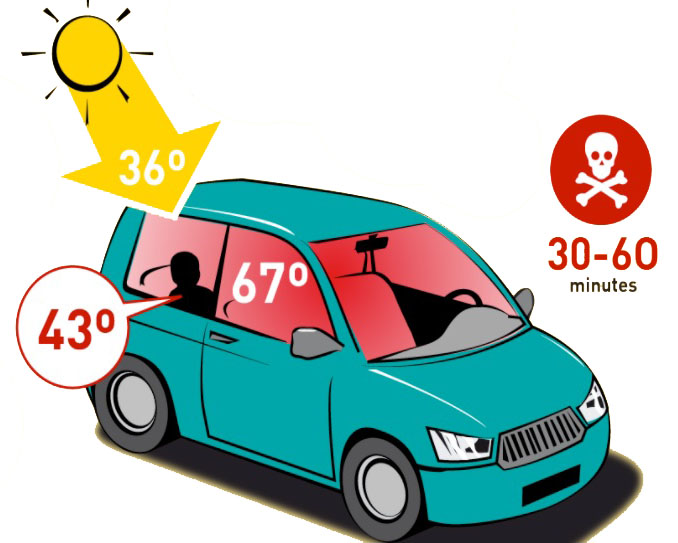
\includegraphics[width=4cm]{Images/hotcar}
	}
	\choice
	{do thể tích khối khí trong ô tô thay đổi nên nhiệt lượng mà khối khí trong ô tô nhận được chủ yếu làm tăng nội năng của khối khí}
	{do thể tích khối khí trong ô tô không đổi nên nhiệt lượng mà khối khí trong ô tô nhận được chủ yếu làm giảm nội năng của khối khí}
	{do thể tích khối khí trong ô tô thay đổi nên nhiệt lượng mà khối khí trong ô tô nhận được chủ yếu làm tăng nội năng của khối khí}
	{\True do thể tích khối khí trong ô tô không đổi nên nhiệt lượng mà khối khí trong ô tô nhận được chủ yếu làm tăng nội năng của khối khí}
	\loigiai{
		Khi ô tô đóng kín cửa và để ngoài trời nắng, bức xạ mặt trời chiếu vào xe qua các cửa kính, gây ra hiệu ứng nhà kính. Nhiệt lượng từ ánh sáng mặt trời làm tăng nội năng của không khí bên trong xe, nhưng thể tích không khí không thay đổi. Do đó, nhiệt độ không khí bên trong ô tô tăng lên đáng kể.
	}
	\haidong{2}\end{ex}
\begin{ex} \nguon{1}
	Lấy hai cốc thủy tinh giống nhau, đổ vào chúng lượng nước cùng nhiệt độ phòng. Cốc đánh dấu số 1 được phủ một miếng vải đen, cốc còn lại là cốc số 2. Đặt cả hai cốc dưới ánh nắng mặt trời và sẽ đo nhiệt độ trong từng cốc. Nhiệt độ trong cốc nào sẽ tăng nhanh hơn?\\
	\centerline{
		
\includegraphics[width=8cm]{images/2024_05_26_010fc85c05a422f9b1ffg-43-01}
	}
	\choice
	{\True Cốc 1}
	{Cốc 2}
	{Bằng nhau}
	{Chưa đủ cơ sở để xác định}
	\loigiai{
		\begin{itemize}
			\item Nhiệt độ nước sẽ tăng nhanh hơn trong cốc được phủ bởi vải đen.
			\item Vì vải đen hấp thụ ánh sáng mặt trời tốt hơn. \item Do đó, cốc được phủ bởi vải đen, được truyền nhiều nhiệt lượng hơn, độ tăng nội năng hơn, sẽ nhanh chóng trở nên nóng hơn, từ đó giúp nước trong cốc nóng lên nhanh hơn bằng cách truyền một phần năng lượng của nó cho nước.\end{itemize}
	}
\end{ex}
\begin{ex} \nguon{4}
	Một người lắc mạnh một phích nước đậy kín trong một thời gian dài. Coi nước trong phích là một hệ kín và không có sự trao đổi nhiệt với môi trường. Khi đó, kết luận nào sau đây là đúng?
		\immini{\choice
		{Nước trong phích không nhận công từ bên ngoài, nội năng của nước không thay đổi}
		{Nước trong phích nhận công từ bên ngoài, nhưng nội năng không thay đổi do không có sự truyền nhiệt}
		{Nước trong phích nhận công từ bên ngoài, nội năng tăng, nhưng nhiệt độ không thay đổi}
		{\True Nước trong phích nhận công từ bên ngoài, nội năng tăng và nhiệt độ cũng tăng}}
	{
\includegraphics[width=2cm]{images/phich}}
	
	\loigiai{
		\begin{enumerate}[label=\alph*)]
			\item Hệ có nhận được công từ bên ngoài thông qua quá trình phích nước được lắc mạnh.
			\item Hệ không nhận nhiệt lượng từ bên ngoài.
			\item Nội năng của hệ sẽ tăng lên do nhận được công từ bên ngoài.
			\item Nhiệt độ của nước sẽ tăng lên do nội năng tăng.
		\end{enumerate}
	}
\end{ex}
\begin{ex}
	\immini[thm]{Xét khối khí như trong hình. Dùng tay ấn mạnh và nhanh pit-tông, vừa nung nóng khí bằng ngọn lửa đèn cồn.
		\choiceTF[t]
		{\True Công $A>0$ vì khí bị nén (khí nhận công)}
		{Nhiệt lượng $Q<0$ vì khí bị nung nóng (khí nhận nhiệt)}
		{\True Nội năng của khí tăng $\Delta U>0$}
		{Biểu thức liên hệ độ biến thiên nội năng, công và nhiệt lượng là $\Delta U=A-Q$}}{
		
\includegraphics[width=2.5cm]{images/2024_05_29_ddddee3750d8eb1e627bg-08}}
	\loigiai{
		\begin{itemchoice}
			\itemch Đ
			\itemch SAI. Khí nhận nhiệt $Q>0$
			\itemch Đ
			\itemch SAI. $\Delta U=A+Q$
		\end{itemchoice}
	}
	\haidong{3}\end{ex}
\begin{ex} \nguon{4}
	\immini[thm]{Động cơ nhiệt là một phát minh vĩ đại của nhân loại, nó mở đầu cho cuộc cách mạng công nghiệp trên thế giới. Động cơ nhiệt là một ứng dụng của định luật I của nhiệt động lực học. Hình bên là sơ đồ nguyên tắc hoạt động của động cơ nhiệt, bên trong động cơ có các tác nhân thực hiện quá trình sinh công (hơi nước, hỗn hợp nhiên liệu khí...).}{ 
\includegraphics[width=3.5cm]{images/2024_05_29_ddddee3750d8eb1e627bg-09}}
	\choiceTF[t]
	{\True Quá trình truyền nhiệt từ nguồn nóng cho tác nhân làm cho nội năng của tác nhân tăng lên}
	{Toàn bộ nhiệt lượng mà tác nhân nhận được từ nguồn nóng đều được biến thành công}
	{\True Nếu không có nguồn lạnh thì nhiệt độ của tác nhân sẽ tăng lên rất nhanh và dẫn đến hỏng động cơ}
	{\True Trong động cơ đốt trong, tác nhân là hỗn hợp khí trộn nhiên liệu trong xilanh}
	\loigiai{
		\begin{itemchoice}
			\itemch ĐÚng
			\itemch Sai. Chỉ một phần nhiệt lượng nhận được từ nguồn nóng chuyển thành công.
			\itemch ĐÚng
			\itemch Đúng
		\end{itemchoice}
	}
\end{ex}